En esta sección se van a evaluar los entornos de desarrollo más populares en el lado del servidor teniendo en cuenta que se va a utilizar React. Si siguiésemos el mismo criterio que con el apartado del lado de cliente, encontraríamos que numerosas fuentes -por ejemplo, \cite{BKETPF1} y \cite{BKETPF2}- están de acuerdo en que PHP es la tecnología más utilizada en el lado de servidor con diferencia. Se puede apreciar en la figura \cref{fig:similartech:backend} sacada de \cite{BKETPF2} en Febrero de 2020. Sin embargo, en este caso particular y por la tecnología elegida en el lado del cliente, se van a valorar positivamente tecnologías que permitan desarrollar al mismo tiempo el cliente y el servidor. PHP es muy utilizado por varias razones:

\begin{enumeration}
	\item Es el más antiguo de los lenguajes de lado de servidor.
	\item Tiene la mayor comunidad que puede tener un lenguaje de servidor y, por tanto, una extensa documentación.
	\item Es utilizado por marcos aun más grandes, como Symphony o Wordpress. Estos son CMS y están fuera del alcance de este proyecto.
\end{enumeration}

Sin embargo, PHP está pensado para directamente renderizar HTML, que es exactamente lo que hace React. Pese a que queremos dar soporte a las tecnologías más extendidas, también queremos estar actualizados con pilas tecnológicas actualizadas y comprobadas. Una de estas pilas tecnológicas de las que hablo es MERN (MongoDB, ExpressJS, ReactJS y NodeJS). Estas pilas tecnológicas están recomendadas por los siguientes motivos:

\begin{enumeration}
	\item Solo hay que aprender un lenguaje, Javascript, lo cual reduce la curva de aprendizaje.
	\item La gestión de datos internos de la aplicación es muy similar a la gestión de base de datos porque MongoDB trabaja con objetos Javascript.
	\item Se pueden hacer contenedores Docker que contengan la pila completa de forma muy sencilla, distribuyendo la carga y haciendo la aplicación escalable. [Faltan citas de todo esto].
\end{enumeration}

Para esto se van a evaluar dos opciones: Express y Next.js. Se ha considerado utilizar múltiples entornos de servidor, entre ellos los que podemos encontrar en la figura \cref{fig:stjs2019:backend}. Sin embargo, teniendo decidido el lado del cliente, la mayoría de opciones no merecen la pena. React trabaja de forma estupenda con NodeJS y lo más habitual es que vayan de la mano. 

\begin{figure}
	\centering
	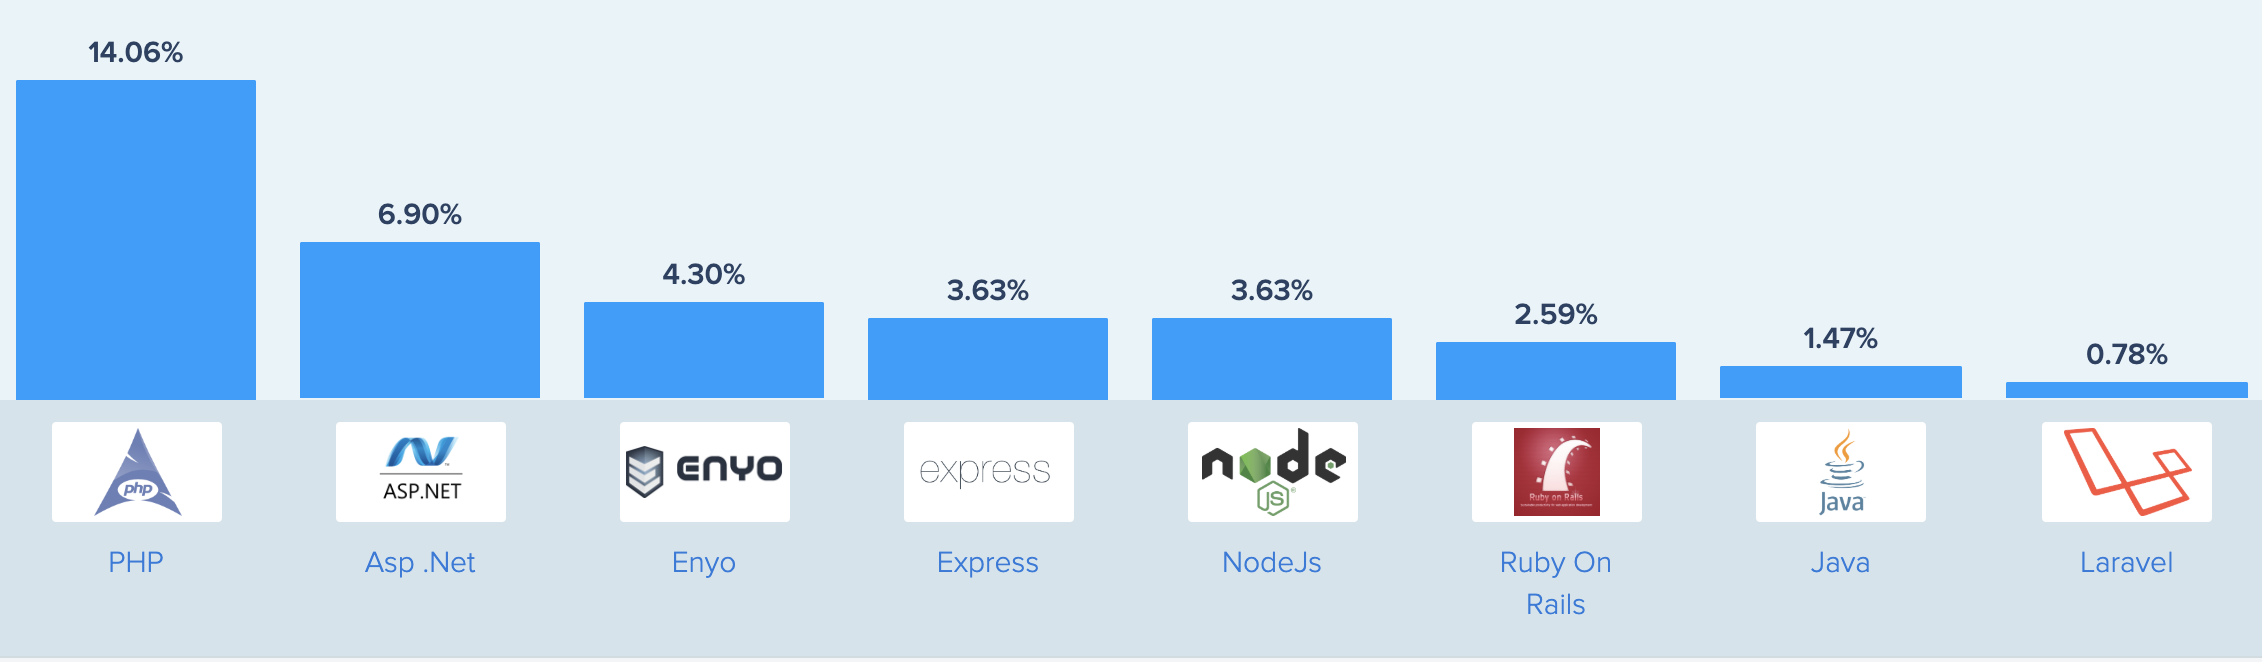
\includegraphics[width=\textwidth]{similartech_backend_trend_top_10K.png}
	\caption{Leading Framework technologies share on the web - Top 10K Sites}
	\label{fig:similartech:backend}
\end{figure}

\begin{figure}
	\centering
	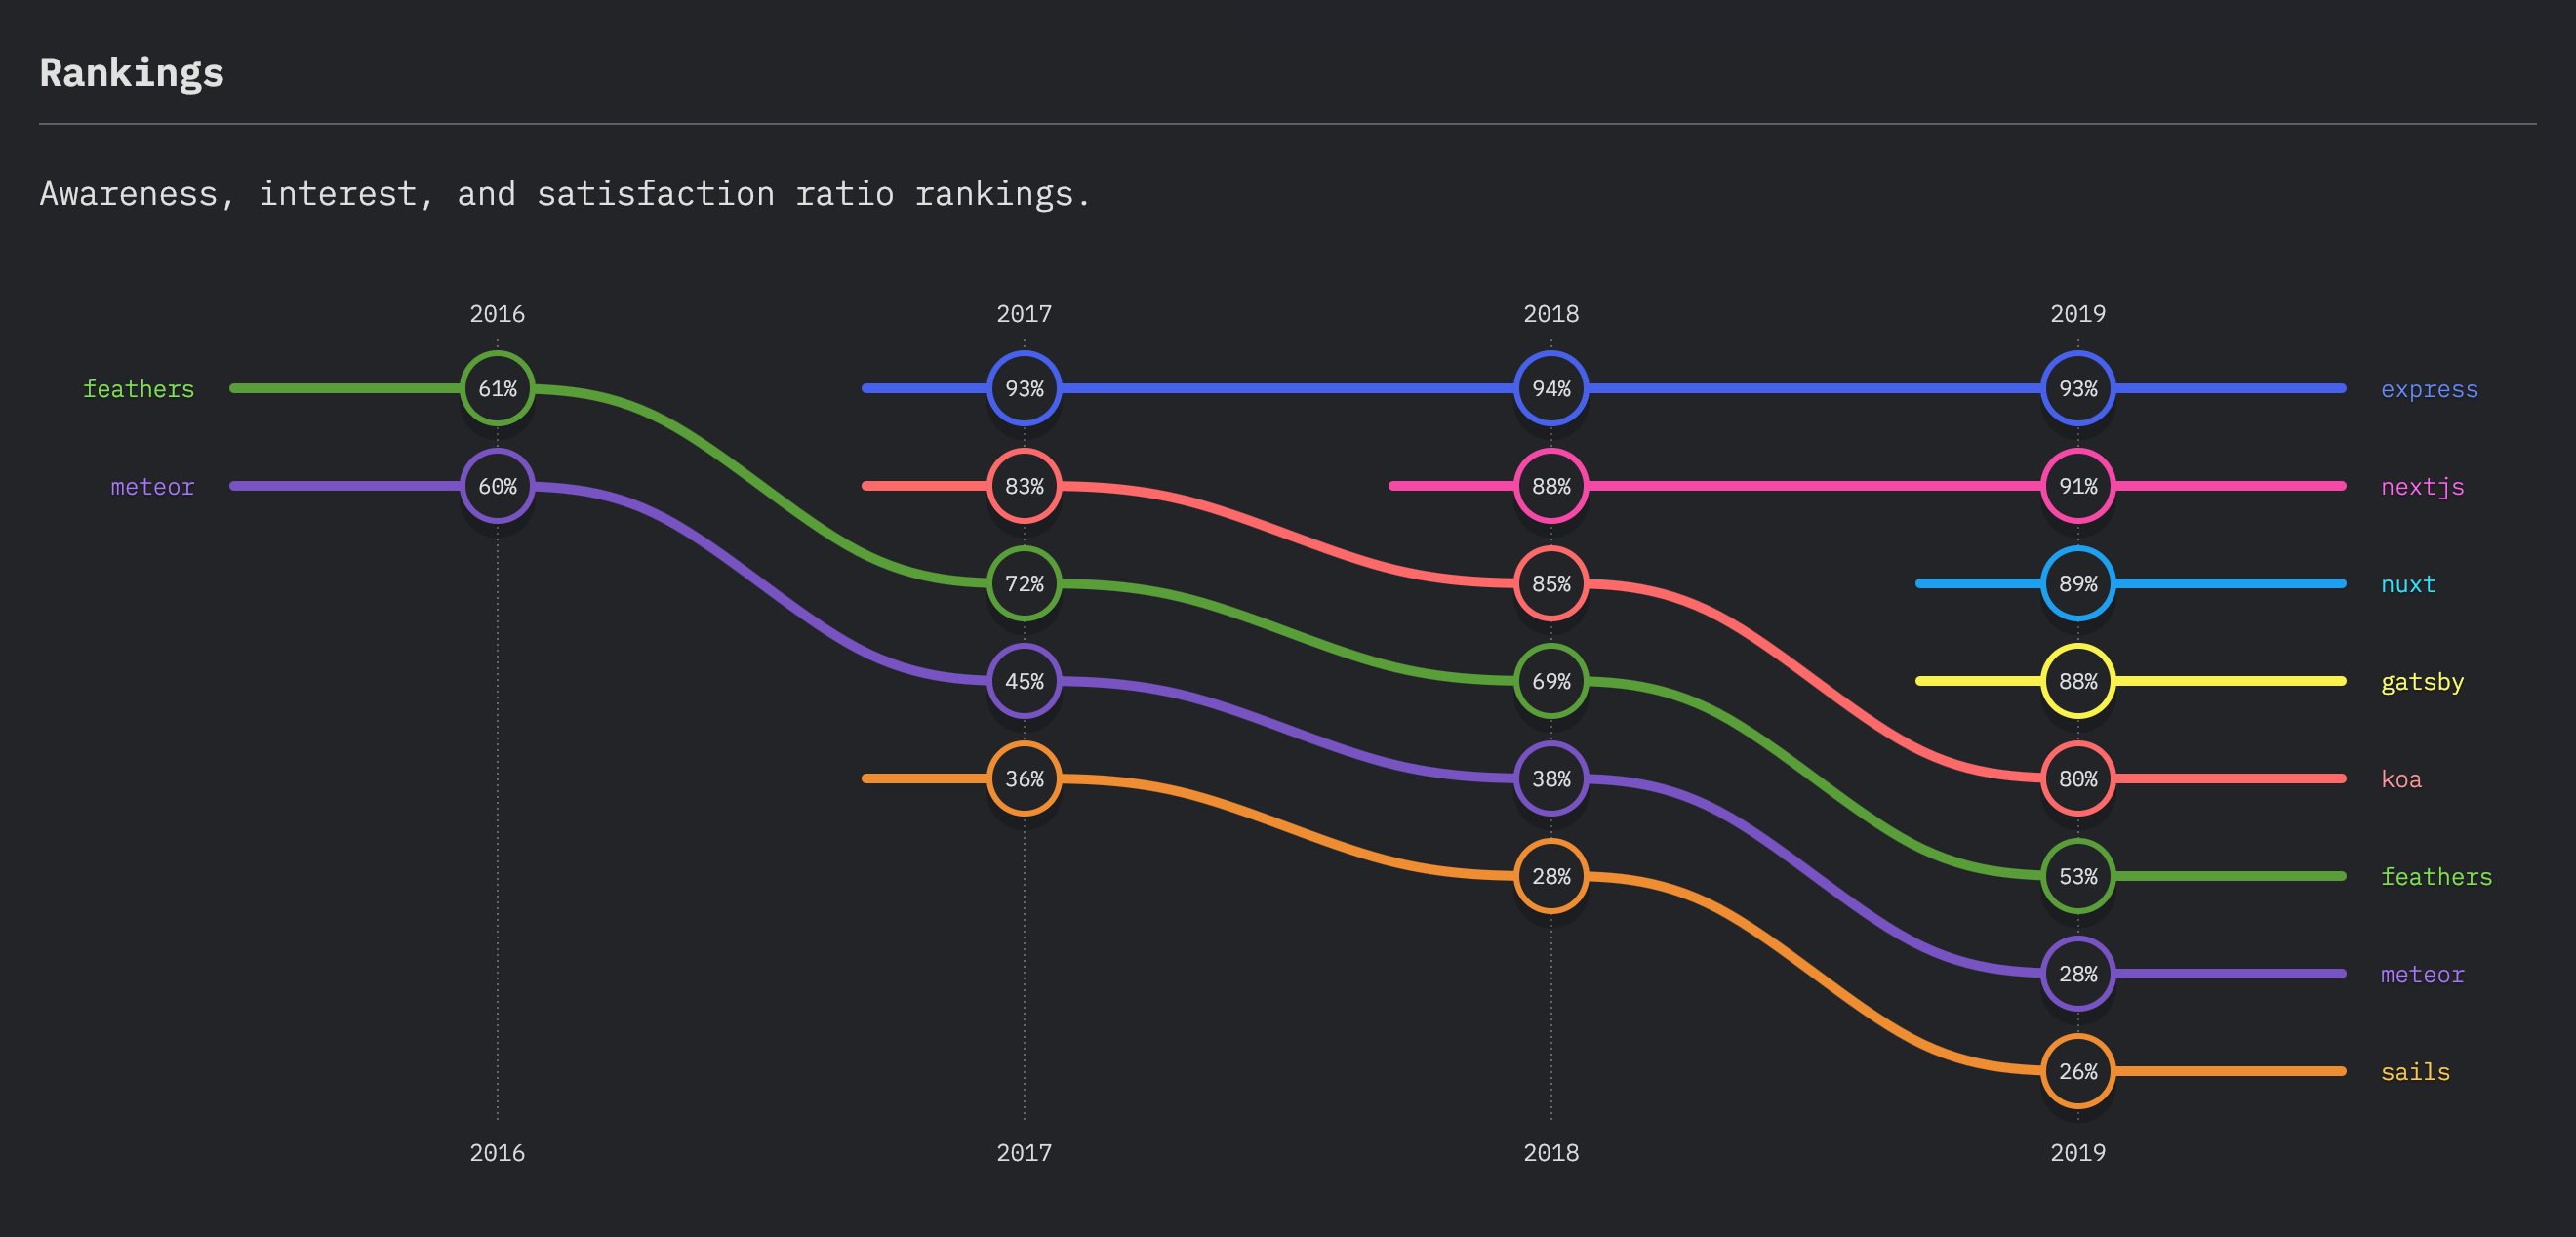
\includegraphics[width=\textwidth]{back_end_frameworks_experience_ranking.png}
	\caption{2019 - Opinión popular de los entornos de trabajo back-end}
	\label{fig:stjs2019:backend}
\end{figure}